\subsection{Reparameterization with SRVT}
\label{subsec:motion-capture-data-reparameterization-srvt}

To find the distance between all motions in the dataset, we use the framework from Chapter \ref{ch:optimal-reparameterization}, which employs reparameterization of the SRVT (Square Root Velocity Transform) of the motions using Algorithm \ref{alg:optimal-reparam-dp} for optimal reparameterization. We then calculate the \(L^2\) distance between the SRVT of the motion and its reparameterized counterpart. This distance is stored in a distance matrix, where the diagonal is zero, as the distance between a motion and itself is zero.

The results are presented as a heatmap to show the unedited results, where the axes represent different motions, and the color indicates the distance between the two motions. These results are shown for various search depths (1, 4, and 10) to demonstrate that higher search depths yield improved outcomes. Ideally, the distance between similar motions should be smaller than the distance between dissimilar motions. Additionally, all motions from the same category should have similar distances to motions from other categories.

The motions are sorted before plotting the heatmap: motions 1-9 are forward jumps, 10-18 are runs/jogs, 19-28 are walks, 29-37 are boxing, and 38-44 are stair climbing. Thus, the heatmap should show blocks of the same color, where the blocks along the diagonal should have close to zero distance.

The results for different search depths using the SRVT method are shown in Figure \ref{fig:heatmaps-dynprog}. In \ref{fig:heatmaps-dynprog-1}, little structure is visible in the heatmap. It appears that the first two motions, "forward jump" and "run/jog," are dissimilar to each other, while the last three motions show some similarity. In \ref{fig:heatmaps-dynprog-4}, we observe four blocks along the diagonal, indicating that "forward jump," "run/jog," "walk," and "climbing stairs" are somewhat distinct. However, there are darker spots indicating some resemblance between walking and climbing stairs. In \ref{fig:heatmaps-dynprog-10}, a similar structure to that of search depth 4 is evident. It is not surprising that "walk" and "climbing stairs" are somewhat similar, as they involve similar motions, with one being on a flat surface and the other on stairs. It appears that boxing is the motion that is hardest for our method to distinguish from the others, which may be intrinsic to the motion itself or may be a limitation of the method.

\begin{figure}
    \centering
    \begin{subfigure}{\textwidth}
        \centering
        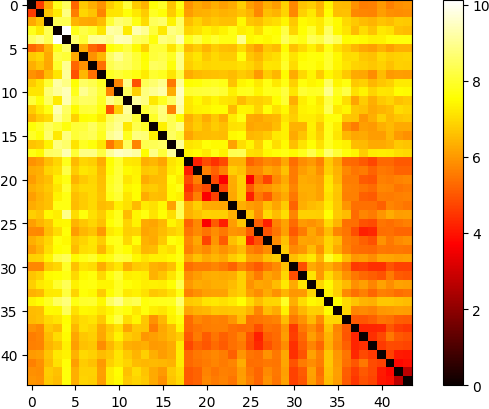
\includegraphics[width=0.53\textwidth]{figures/motion-capture-data/heatmaps/dynprog_1.png}
        \caption{}
        \label{fig:heatmaps-dynprog-1}
    \end{subfigure}
    \begin{subfigure}{\textwidth}
        \centering
        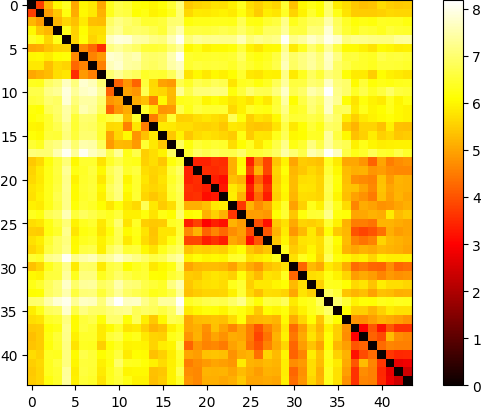
\includegraphics[width=0.53\textwidth]{figures/motion-capture-data/heatmaps/dynprog_4.png}
        \caption{}
        \label{fig:heatmaps-dynprog-4}
    \end{subfigure}
    \begin{subfigure}{\textwidth}
        \centering
        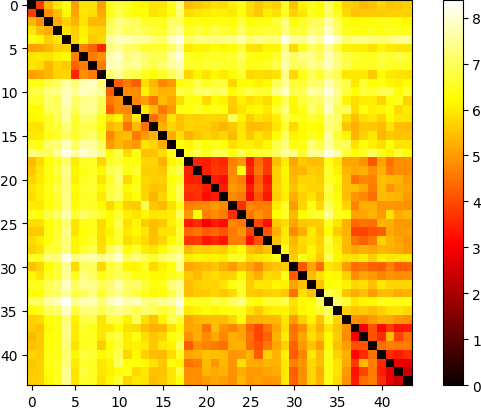
\includegraphics[width=0.53\textwidth]{figures/motion-capture-data/heatmaps/dynprog_10.png}
        \caption{}
        \label{fig:heatmaps-dynprog-10}
    \end{subfigure}
    \caption[Heatmap: Motion Capture Data Classification utilizing Reparameterization]{Heatmaps of the distance matrix from motion capture data, where the distance matrix was created by reparameterization using dynamic programming and search depths of: (a) 1, (b) 4, and (c) 10.}
    \label{fig:heatmaps-dynprog}
\end{figure}